\documentclass[notitlepage,letterpaper, 11pt]{article}
\usepackage[spanish]{babel}
\usepackage[left=3.00cm, right=2.5cm, top=3.50cm, headheight=14pt]{geometry}
\usepackage{pdfpages}


% Datos de la portada
\title{Premio Turing \textbar \hspace{.1mm} A.M. Turing Award}
\author{Rodrigo R. Rubio Haro}
\date{\today} %

\begin{document}
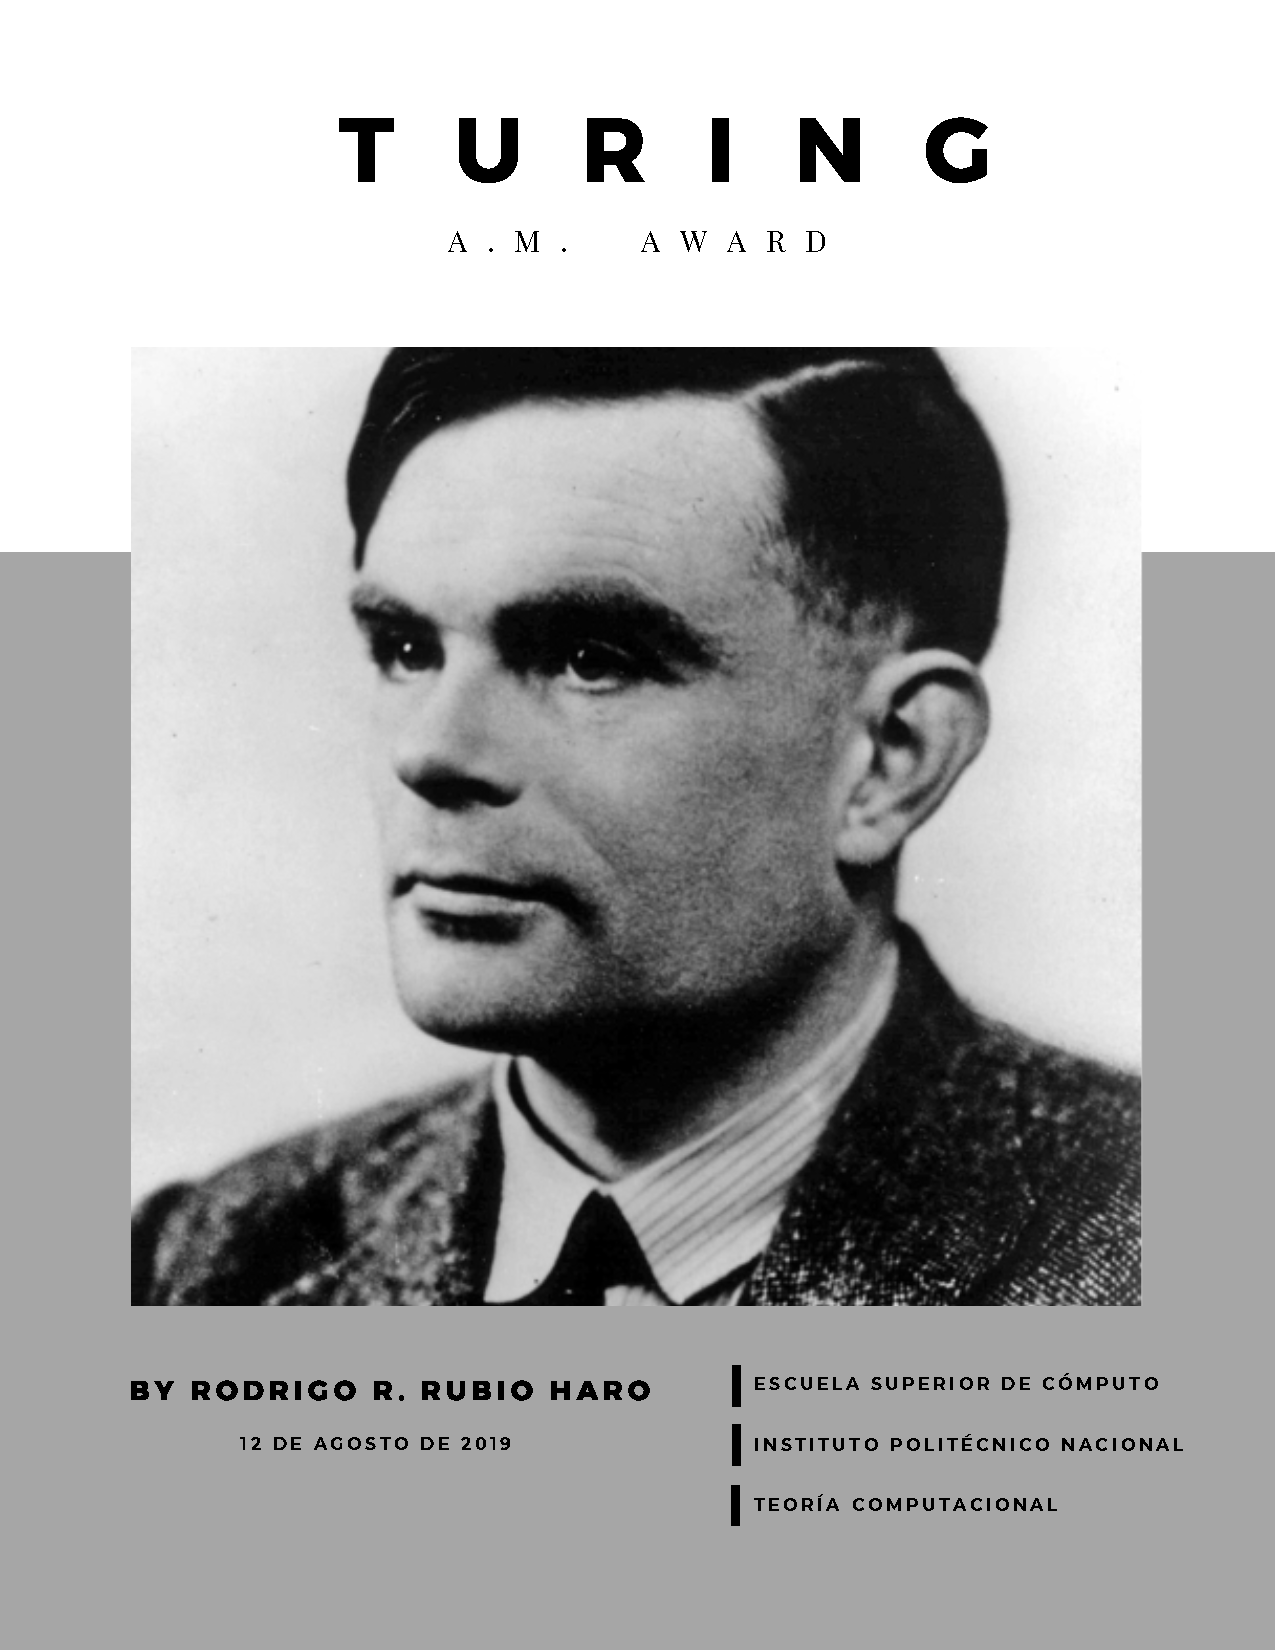
\includepdf{portada.pdf}
\newpage

\section*{Introducción}
El premio Turing, a veces referido como el ``Nobel de la Computación", recibe el nombre en honor del Matemático y Científico Británico, Alan Mathison Turing (1912-1954). Avances fundamentales en arquitectura computacional, complejos algoritmos, inteligencia artificial y formalización de la Computación son tan solo unos de sus logros y áreas de estudio. Reconocido por su papel en la segunda guerra mundial en el área de criptografía. Con dudosas causas de muerte, el veredicto fue suicidio, envenenamiento por cianuro, encontrado en junio de 1945. Después de ser llevado a juicio por relaciones homosexuales en la ciudad de Manchester.
Patrocinado por Alphabet Inc. (Antes Google Inc.) es premio más prestigioso que la Asociación de Maquinaria Computacional (ACM, por sus siglas en inglés) otorga a las contribuciones más trascendentales e importantes en materia de Computación.


\section*{Lista de premios Turing}

\section*{1966 - Perlis, Alan J.}
\noindent Pennsylvania, 1922. Nace Alan en Pittsburgh, Estados Unidos.

\noindent Ganador del premio por su influencia en el área de técnicas de programación avanzada y construcción de Compiladores. Véase ``The Synthesis of Algorithmic Systems". 

\noindent Áreas de estudio: Compiladores y programación

\noindent Muere en febrero de 1990, en connecticut, Estados Unidos.
\newline

\section*{1967 - Maurice V. Wilkes.}
\noindent Dudley, 1913. Maurice Vicent Wilkes en Inglaterra, Reino Unido. 

\noindent Ganador del premio por diseñar la EDSAC, la primera computadora con un programa almacenado y por su coautoría en ``Preparación de programas para computadoras digitales electrónicas". Véase ``The Computers Then and Now ".

\noindent Áreas de estudio: Hardware y Arquitectura Computacional

\noindent Muere en noviembre de 2010, en Cambriedge, Reino Unido.
\newline

\section*{1968 - Richard W. Hamming.}
\noindent Chicago, 1915. Nace Richard en Illinois, Estados Unidos.

\noindent Ganador del premio por su trabajo en métodos numéricos, códigos de codificación automática, detección y corrección de errores. 

\noindent Áreas de estudio: Códigos de Corrección de Errores y Métodos Numéricos.

\noindent Muere en enero de 1998, en California, Estados Unidos.
\newline


\section*{1969 - Marvin Minsky}
\noindent New York City, 1927. Nace Marvin en Estados Unidos.

\noindent Ganador del premio por su excepcional trabajo en inteligencia artificial. Véase ``Form and Content in Computer Science"

\noindent Área de estudio: Inteligencia artificial.

\noindent Muere en enero de 1998, en California, Estados Unidos.
\newline


\section*{1970 - James Hardy Wilkinson}
\noindent Strood, 1927. Nace Jim en Inglaterra, Reino Unido.

\noindent Ganador del premio por su investigación en análisis numérico para facilitar el uso de computadoras digitales de alta velocidad. Reconocido por su trabajo en álgebra lineal y análisis de errores "backward". Véase ``Some Comments from a Numerical Analyst"

\noindent Área de estudio: Análisis Numérico

\noindent Muere en octubre de 1986, en Teddington, Reino Unido.
\newline

\section*{1971 - John McCarthy}
\noindent Boston, 1927. Nace el inventor del lenguaje de programación LISP el Dr. McCarthy en Massachusetts, Estados Unidos.

\noindent Ganador del premio por sus aportaciones en inteligencia artificial.Véase ``Estado Actual de la Investigación en Inteligencia Artificial"

\noindent Área de estudio: Inteligencia artificial.

\noindent Muere en octubre de 1986, en Standford, Estados Unidos.
\newline

\section*{1972 - Edsger Wybe Dijkstra}
\noindent Rotterdam, 1930. Nace el científico Edsger Dijkstra en los Países Bajos.

\noindent Ganador del premio por sus contribuciones en la programación como reto intelectual, la demostración de que los programas deben componerse correctamente no solo corregidos. Véase ``The Humble Programmer".

\noindent Área de estudio: Verificación de programas.

\noindent Muere en agosto de 2002, en Nuenen, Países Bajos.
\newpage

\section*{1973 - Charles William Bachman}
\noindent Manhattan, 1924. Nace Charles William en Kansas, Estados Unidos.

\noindent Ganador del premio por sus sobresalientes contribuciones a la tecnología de las bases de datos, de los pocos no ``académicos" ganadores del premio.

\noindent Área de estudio: Bases de Datos.

\noindent Muere en julio de 2017.
\newline

\section*{1974 - Donald Knuth}
\noindent Milwaukee, 1930. Nace Donald Ervin Knuth en Wisconsin, Estados Unidos.

\noindent Ganador del premio por sus contribuciones en el diseño de lenguajes de programación y el análisis de algoritmos; y en lo particular, por su serie de libros ``El arte de programar computadoras".

\noindent Áreas de estudio: Análisis de algoritmos y Programación.
\newline

\section*{1975 - Newell Alle y Simon Herbert}
\noindent Ambos Estadounidenses, Newell Alle y Herbert Alexander Simon, ganan el premio Turing por sus contribuciones fundamentales a la Inteligencia Artificial, a la sicología de la condición humana y el procesamiento de listas. Véase ``Computer Science as Empirical Inquiry:
Symbols and Search".

\noindent Áreas de estudio: Inteligencia Artificial y Procesamiento de Listas
\newline

\section*{1976 - Michael O. Rabin y Dana Stewart Scott}
\noindent El duo germano-estadounidense gana el premio Turing por su trabajo ``Autómatas finitos y sus problemas de toma de decisiones", con la valiosa idea de maquinas no deterministas.

\noindent Áreas de estudio: Teoría computacional y Autómatas finitos
\newline

\section*{1977 - John Backus}
\noindent Philadelphia, 1924. Nace John Backus en Pennsylvania, Estados Unidos.

\noindent Ganador del premio por sus contribuciones profundas, influyentes y trascendentes al diseño de sistemas prácticos de alto nivel. Su trabajo en FORTRAN y la publicación de procedimientos formales para la especificación de lenguajes de programación.

\noindent Área de estudio: Programación y Lenguajes de Programación.

\noindent Muere en marzo de 2007 en Oregon, Estados Unidos.
\newline

\section*{1978 - Robert W. Floyd}
\noindent New York, 1936. Nace Bob Floyd en Estados Unidos.

\noindent Ganador del premio por su influencia en metodologías de creación de software eficiente y confiable, fundador de los subcampos de ciencias de la computación: Teoría del análisis, Verificación y síntesis automática de Programas; y Análisis de algoritmos. 

\noindent Área de estudio: Software.

\noindent Muere en septiembre de 2001 en California, Estados Unidos.
\newline

\section*{1979 - Kenneth E. Iverson}
\noindent Camrose, 1936. Nace Kenneth Eugene Iverson en Alaberta, Canadá.

\noindent Ganador del premio por ser pionero en lenguajes de programación y notación matemática, resultando en el lenguaje APL.

\noindent Área de estudio: Lenguajes de programación.

\noindent Muere en octubre de 2004 en Ontario, Canadá.
\newline

\section*{1980 - C. Antony R. Hoare}
\noindent Nace en 1934 Charles Antony Richard Hoare en la República Democrática Socialista de Sri Lanka.

\noindent Ganador del premio por ser su contribución en la definición y diseño de los lenguajes de programación.

\noindent Área de estudio: Lenguajes de programación.
\newline

\section*{1981 - Edgar F. Codd}
\noindent Portland, 1936. Nace Edgar Frank (Ted) Codd en Inglaterra, Reino Unido.

\noindent Ganador del premio por sus continuas contribuciones, teóricas y prácticas, en sistemas de gestión de bases de datos. 

\noindent Área de estudio: Bases de datos.

\noindent Muere en abril de 2003 en Florida, Estados Unidos.
\newpage

\section*{1982 - Stephen Arthur Cook}
\noindent Buffalo NY, 1939. Nace Stephen Arthur Cook en Estados Unidoss.

\noindent Ganador del premio por su avance en el entendimiento de la complejidad de la computación de una manera profunda y significativa. Su trabajo ``La complejidad de los procedimientos de prueba de teoremas" sentó las bases de la teroría NP-completo sobre procesos de decisiones.

\noindent Área de estudio: Complejidad computacional.
\newline

\section*{1983 - Ritchie, Dennis M. y Thompson, Kenneth Lane}
\noindent Ambos estadounidenses ganan el premio Turing por su trabajo en teoría de los sistemas operativos y más especificamente por la implementación del sistema operativo UNIX.

\noindent Área de estudio: Sistemas operativos.
\newline

\section*{1984 - Niklaus E. Wirth}
\noindent Winterhur, 1936. Nace Niklaus Wirth en Suecia.

\noindent Ganador del premio por su trabajo en EULER, ALGOLW, MODUL y PASCAL.

\noindent Área de estudio: Lenguajes de programación.
\newline

\section*{1985 - Richard Manning Karp}
\noindent Boston, 1936. Nace Richard Manning Karp en Massachusetts, Estados Unidos.

\noindent Ganador del premio por sus contribuciones a la teoría de algoritmos, incluyendo algoritmos para flujo de red asi como problemas de optimización combinatoria.

\noindent Área de estudio: Algoritmos de combinatoria.
\newline

\section*{1986 - Hopcroft, John E. y Tarjan, Robert (Bob) Endre}
\noindent Ambos estadounidenses ganan el premio Turing por sus logros fundamentales en el diseño y análisis; de algoritmos y estructuras de datos.

\noindent Áreas de estudio: Análisis de algoritmos y Estructuras de datos.
\newpage

\section*{1987 - John Cocke}
\noindent Carolina del norte, 1925. Nace John Cocke en los Estados Unidos.

\noindent Ganador del premio por su trabajo en la teroría y diseño de los compiladores.

\noindent Áreas de estudio: Compiladores y Arquitectura de las computadoras.

\noindent Muere en julio de 2002 en New York, Estados Unidos.
\newline

\section*{1988 - Sutherland, Ivan E.}
\noindent Hastings, 1938. Nace Ivan Edward Sutherland en Nebraska, Estados Unidos.

\noindent Ganador del premio por su trabajo en gráficos de computadoras que inicio con el programa de dibujo Sketchpad

\noindent Área de estudio: Gráficos.
\newline

\section*{1989 - William Kahan.}
\noindent Toronto, 1933. Nace William (Velvel) Morton Kahan en Ontario, Canadá.

\noindent Ganador del premio por sus contribuciones fundamentales en el análisis numérico. Reconocido por ser experto en el cálculo flotante.

\noindent Área de estudio: Análisis numérico.
\newline

\section*{1990 - Fernando J. Corbato}
\noindent Oakland, 1926. Nace Fernando José Corbató (Corby) en California, Estados Unidos.

\noindent Ganador del premio por su trabajo pionero en el desarrollo de sistemas informáticos de uso general, a gran escala, de tiempo y recursos compartidos. 

\noindent Área de estudio: Sistemas informáticos.
\newpage

\section*{1991 - Arthur John R. G. Milner}
\noindent Yealmpton, 1925. Nace Arthur John Robin Gorell Milner en los Inglaterra, Reino Unido.

\noindent Ganador del premio por el desarrollo del sistema LCF, una de las primeras herramientas de demostración automática de teoremas. También desarrolló ML, que era el meta lenguaje para escribir estrategias y tácticas en LCF. También fue el primer lenguaje en poseer un sistema polimórfico de tipos con inferencia automatizada y manejo de excepciones seguro desde el punto de vista de tipos.
Y por ultimo, desarrolló un marco teórico para el análisis de sistemas concurrentes, el cálculo de sistemas comunicantes y su sucesor, el cálculo pi.


\noindent Áreas de estudio: Lenguajes de programación asi coomo la construcción de pruebas.

\noindent Muere en marzo de 2010 en Cambriedge, Inglaterra.
\newline

\section*{1992 - Butler W Lampson}
\noindent Washington D.C., 1943. Nace Butler Lampson en los Estados Unidos.

\noindent Ganador del premio por sus contribuciones al desarrollo de entornos informáticos personales distribuidos y la tecnología para su implementación: estaciones de trabajo, redes, sistemas operativos, sistemas de programación, pantallas, seguridad y publicación de documentos.


\noindent Área de estudio: Computadoras personales.
\newline

\section*{1993 - Juris Hartmanis y Richard Edwin}
\noindent Richard Edwin Stearns de New Jersey, Estados Unidos y Juris Hartmanis de Riga, capital de Letonia ganan el premio Turing por su trabajo, que estableció los fundamentos del campo de la teoría de la complejidad computacional.

\noindent Área de estudio: Complejidad computacional.
\newline


\section*{1994 - Edward A Feigenbaum y Dabbala Rajagopal Reddy}
\noindent Edward Feigenbaum de New Jersey, Estados Unidos y Raj Reddy de Katoor, India ganan el premio Turing por ser pioneros en el diseño y construcción a gran escala de sistemas de inteligencia artificial, demostrando el potencial económico de esta tecnología.

\noindent Área de estudio: Inteligencia Artificial.
\newpage

\section*{1995 - Manuel Blum}
\noindent Caracas, 1938. Nace Manuel Blum en Venezuela.

\noindent Ganador del premio Turing por sus contribuciones a los fundamentos de la teroría de la complejidad computacional y su aplicación a la criptografía.

\noindent Áreas de estudio: Criptografía y complejidad computacional.
\newline

\section*{1996 - Amir Pnueli}
\noindent Nahalal, 1941. Nace Amir Pnueli en Israel.

\noindent Ganador del premio Turing por la introducción de la lógica temporal en la computación y por sus extraordinarias contribuciones a la verificación de sistemas.

\noindent Área de estudio: Verificación de programas. 
\newline

\section*{1997 - Douglas Engelbart}
\noindent Portland, 1925. Nace Douglas Engelbart en Oregon, Estados Unidos.

\noindent Ganador del premio Turing por su inspiradora visión de la computación interactiva y asi como la tecnología para hacerlo posible.

\noindent Área de estudio: Computación interactiva. 

\noindent Muere en julio de 2013 en Oregon, Estados Unidos.
\newline


\section*{1998 - James Nicholas Gray}
\noindent San Francisco, 1944. Nace James Gray en California, Estados Unidos.

\noindent Ganador del premio Turing por sus contribuciones fundamentales a la investigación de procesamiento de bases de datos y transacciones y liderazgo técnico en la implementación del sistemas.

\noindent Área de estudio: Bases de datos. 

\noindent Desaparece en su velero en 2007 y es declarado muerto en enero de 2012 (5 años después) en San Francisco, Estados Unidos.
\newline

\section*{1999 - Frederick Brooks}
\noindent Carolina del norte, 1931. Nace Frederick Phillips Brooks en los Estados Unidos.

\noindent Ganador del premio Turing por sus contribuciones históricas en las arquitecturas computacionales, sistemas operativos y en la ingenieria de software.

\noindent Áreas de estudio: Arquitectura de computadoras, Sistemas operativos e ingenieria de software. 
\newline

\section*{2000 - Andrew Chi-Chih Yao}
\noindent Shangai, 1946. Nace Andrew en China.

\noindent Ganador del premio Turing por sus contribuciones en la Teoría de la computación, criptografía y complejidad de la comunicación.

\noindent Área de estudio: Criptografía. 
\newline


\section*{2001 - Ole-Johan Dahl y Kristen Nygaard}
\noindent Ole-Johan Dahl de Mandal, Noruega y Kristen Nygaard  de Oslo, Noruega  ganan el premio Turing por ser pilares en la creacion del paradigma de Programación Orientada a Objetos.

\noindent Área de estudio: Programación Orientada a Objetos.
\newline

\section*{2002 - Leonard Max Adleman; Ronald Linn Rivest y Adi Shamir}
\noindent Leonard Max Adleman de San Francisco, Estados Unidos; Adi Shamir de Tel Aviv, Israel y  Ronald Linn Rivest de New York, Estados Unidos  ganan el premio Turing por su ingenio y contribución de hacer las llaves publicas utiles en la practica.

\noindent Área de estudio: Criptografía.
\newline

\section*{2003 - Alan Curtis Kay}
\noindent Springfield, 1940. Nace Alan Curtis Kay en Massachusetts, Estados Unidos.

\noindent Ganador del premio Turing por sus contribuciones en lenguajes de programación orientada a objetos modernos y por contribuciones fundamentales en la computación personal.

\noindent Áreas de estudio: Computadoras personales y Lenguajes de programación.
\newline

\section*{2004 - Vinton Gray Cerf y Robert Elliot Kahn}
\noindent Ambos estadounidenses  ganan el premio Turing por su trabajo en la Internet, incluyendo protocolos de comunicación como TCP/IP.

\noindent Área de estudio: Comunicaciones en Internet.
\newpage

\section*{2005 - Peter Naur}
\noindent Frederiksberg, 1928. Nace Peter Naur en Dinamarca.

\noindent Ganador del premio Turing por sus contribuciones al diseño de lenguajes de programación, diseño de compiladores y al arte y practica de la programación.

\noindent Área de estudio: Lenguajes de programación.

\noindent Muere en enero de 2016 en Herlev, Dinamarca.
\newline

\section*{2006 - Frances Elizabeth Allen}
\noindent Peru, New York, 1932. Nace Frances Elizabeth en los Estados Unidos.

\noindent Ganador del premio Turing por sus contribuciones a la teoría y práctica de optimización de técnicas de compilación, bases de ejecución automática en paralelo y de la optimización de compiladores moderna.

\noindent Área de estudio: Compiladores.
\newline

\section*{2007 - Edmund Melson Clarke, E. Allen Emerson y Joseph Sifakis}
\noindent Francia y Estados Unidos compartieron el premio con los científicos Edmund Melson Clarke, E. Allen Emerson (ambos estadounidenses) y Joseph Sifakis (naturalizado francés) por su desarrollo del modelo Model-Checking, tecnología de verificación altamente efectiva que es ampliamente adoptada en la industria.

\noindent Áreas de estudio: Verificación de modelos de software y hardware.
\newline

\section*{2008 - Barbara Liskov}
\noindent California, 1939. Nace Barbara Liskov en los Estados Unidos.

\noindent Ganador del premio Turing por su trabajo en temas como la abtracción de los datos, tolerancia a las fallas y sistemas distribuidos.

\noindent Áreas de estudio: Sistemas operativos y lenguajes de programación.
\newline

\section*{2009 - Chuck Thacker}
\noindent Passadena, California, 1943. Nace Chuck en los Estados Unidos.

\noindent Ganador del premio Turing por el diseño y el desarrollo de la primera computadora personal moderna, entre otras contribuciones como en las redes LAN.

\noindent Áreas de estudio: Arquitectura computacional y computadoras personales.
\newline

\section*{2010 - Leslie Gabriel Valiant}
\noindent Budapest, 1949. Nace Les Valiant en Hungría.

\noindent Ganador del premio Turing por sus aportes trascendentales en teoría de la computación, aprendizaje computacional, resaltando el aprendizaje correcto probablemente aproximado (Aprendizaje PAC, por sus siglas en inglés), así como computación algebraica, paralela y distribuida.

\noindent Áreas de estudio: Inteligencia artificial, complejidad computacional, machine learning y computación paralela.
\newline

\section*{2011 - Judea Pearl}
\noindent Tel Aviv, 1936. Nace Judea Pearl en Israel.

\noindent Ganador del premio Turing por sus contribuciones fundamentales a la inteligencia artificial, desarrollando un calculo para el razonamiento probabilístico.

\noindent Áreas de estudio: Inteligencia artificial y Análisis de algoritmos.
\newline

\section*{2012 - Silvio Micali y Shafi Goldwasser}
\noindent Israel y Estados Unidos compartieron el premio con los científicos Silvio Micali y Shafi Goldwasser por su trabajo en la ciencia de la criptografía y por sus nuevos métodos para la verificación de pruebas matemáticas de la teoría de la complejidad.

\noindent Área de estudio: Complejidad computacional y Criptografía.
\newline

\section*{2013 - Leslie Lamport}
\noindent New York, 1941. Nace Leslie Lamport en los Estados Unidos.

\noindent Ganador del premio Turing por sus contribuciones fundamentales en la teoría y práctica de sistemas distribuidos y concurrentes.

\noindent Áreas de estudio: Lenguajes de programación y Análisis de algoritmos.
\newline

\section*{2014 - Michael Stonebraker}
\noindent Massachusetts, 1943. Nace Michael Stonebraker en los Estados Unidos.

\noindent Ganador del premio Turing por la introducción de conceptos y practicas en sistemas de bases de datos modernos.

\noindent Áreas de estudio: Bases de datos y Software.
\newline

\section*{2015 - Whitfield Diffie y Martin Hellman}
\noindent Ambos estadounidenses, ganan el premio Turing por la invención de la criptografía asimétrica de llaves publicas, así como su aplicación a las firmas digitales, como un método practico para el intercambio de llaves.

\noindent Áreas de estudio: Bases de datos y Software.
\newline

\section*{2016 - Tim Berners-Lee}
\noindent Londres, 1955. Nace Tim Berners-Lee en Inglaterra.

\noindent Ganador del premio Turing por inventar la gran red ``world wide web", asi como el primer navegador web y los protocolos que permitirían escalar la gran red.
\newline

\section*{2017 - John L. Hennessy y David Patterson}
\noindent Ambos estadounidenses, ganan el premio Turing por el enfoque sistemático y cuantitativo para el diseño y la evaluación de arquitecturas computacionales, y su impacto en la industria de los microprocesadores.
\newline


\section*{2018 - Yoshua Bengio, Geoffrey E. Hinton y Yann LeCun}
\noindent Canadá y Estados unidos comparten el Turing con Yoshua Bengio, Geoffrey E. Hinton (Canadienses) y Yann LeCun (estadounidense) por su trabajo en las redes neuronales como componentes críticos de la computación.
\newline

\section*{2019 - ?}
\noindent La inteligencia artificial ha ocupado encabezados de numerosos periódicos, y sin duda ha sido una materia de reconocimiento en los A.M. Turing Award, confio que en las ediciones venideras veremos increíbles avances en la implementación y uso de estas tecnologías. 
\newline

``Sólo podemos ver poco del futuro, pero lo suficiente para darnos cuenta de que hay mucho que hacer.''

\rightline{{ --- Alan Turing}}

\begin{thebibliography}{*}
    \bibitem{Tring} A.M. Turing Award. (n.d.). Obtenido Agosto 12, 2019, de https://amturing.acm.org/
    \end{thebibliography}

\end{document}
